\chapter{Spatio-temporal movement patterns}\label{hernoemen}


\section{Introduction}
% count the aggregated movement between building and movement between buildings and world over certain time period
% 2 types of movement visualization : 1) maps; 2) charts
Movement patterns are defined as how people regularly move on the campus. To answer this question, there are two sub questions to answer: when do people move, from where do they move and where do they move to. These patterns consists of spatial component and temporal component, thus they are called spatio-temporal movement patterns.

Movement pattern is actually a kind of behavior pattern, which implicitly reveal how people use the campus and furthermore how they think and behave. In this chapter, several patterns related to time and space are going to be discussed on building level. These movement patterns are about how and when  people move between different buildings, and according to these movement patterns, the reason why people move in this way at a certain time can be explored.

In this chapter, \autoref{chapter9methods} will discuss the methodology of exploring the movement patterns, mainly in four ways: all movements, mobile and static devices, week and weekend and from or to a building duiring a time period. First in \autoref{chapter9Allmovement}, all movements in the database are described regardless of any time or spatial components, then in \autoref{chapter9mobilestatic}, the difference of movements between mobile devices and static devices will be discussed. In \autoref{chapter9weekweekend}, temporal component is taken into consideration, the movement patterns in week days and weekends are going to be described. Finally in \autoref{chapter9fromto}, movements from or to a building in a time period will be explored. 

\section{Methods}\label{chapter9methods}
% states to movements
% GUI for visual exploration of the data and movement patterns
% Final visualization method

A state/stay place is defined as a time interval during which a particular device is located in a certain area, and movement is from the location of one state to the location of another state. In building level, movement is defined as a state between two successive scans in different two buildings.
In database, one movement record contains the start time of the movement, the end time of the movement, the start building, the end building and whether a device is labeled as mobile device or static device. With time information, it is easy to distinguish week days and weekends, and look for movements only in a certain time interval. And with building information, movement pattern from or to one specific building can be found. With attribute 'type', static devices can be filtered out so that only mobile devices are kept in order to make results more reliable. Besides, the difference between movements of static devices and mobile devices can also be explored.

In order to find movement patterns, a GUI is made for automatic visual exploration of the data and movement patterns. For the following four topics, there are both graphs and maps to describe movement patterns. The graphs show the movement in time from 6:00 to 0:00 and the maps show the amount of movements between buildings. The movements are shown in straight lines between buildings because the space of the campus is not constraint, it is not possible to know how exactly people move from building to another building, so that snapping the movements to the road network might give the readers wrong impression. The line width represents the amount of movements, the thicker the line is, the more movements there are. Besides, the color of the line also stresses the amount of movements, where red represents the most movements.

\section{Results}\label{chapter9results}
\subsection{All movement}\label{chapter9Allmovement}

\begin{figure}[H]
	\centering
	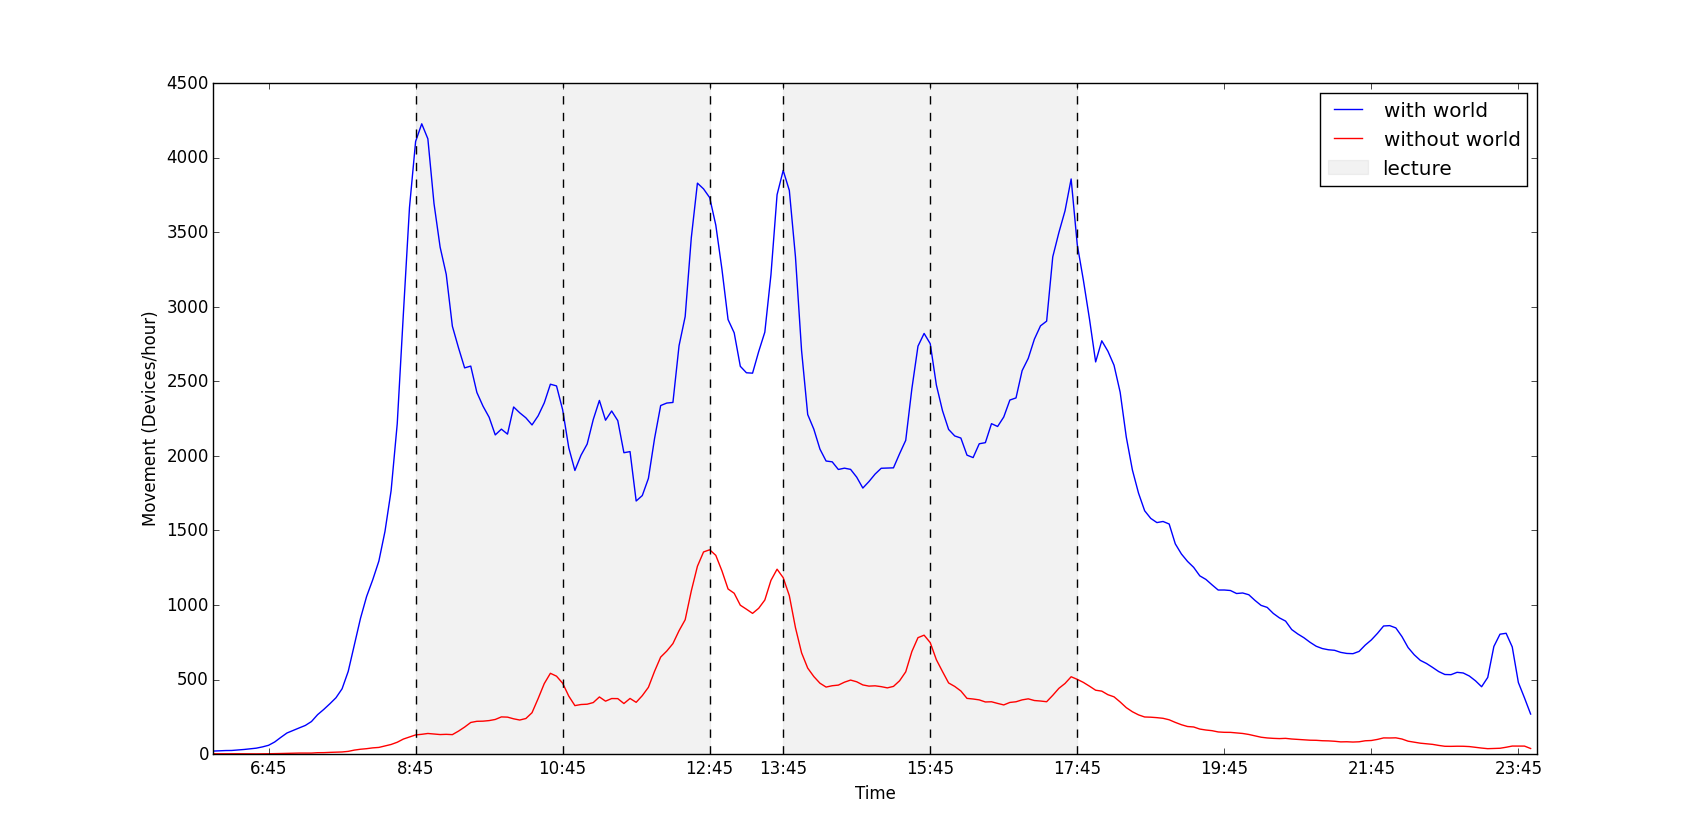
\includegraphics[scale=0.3]{building_all_graph.png}
	\captionsetup{justification=centering}
	\caption{Graph of all movements}
	\label{building_all_graph}
\end{figure}

\begin{figure}[H]
	\centering
	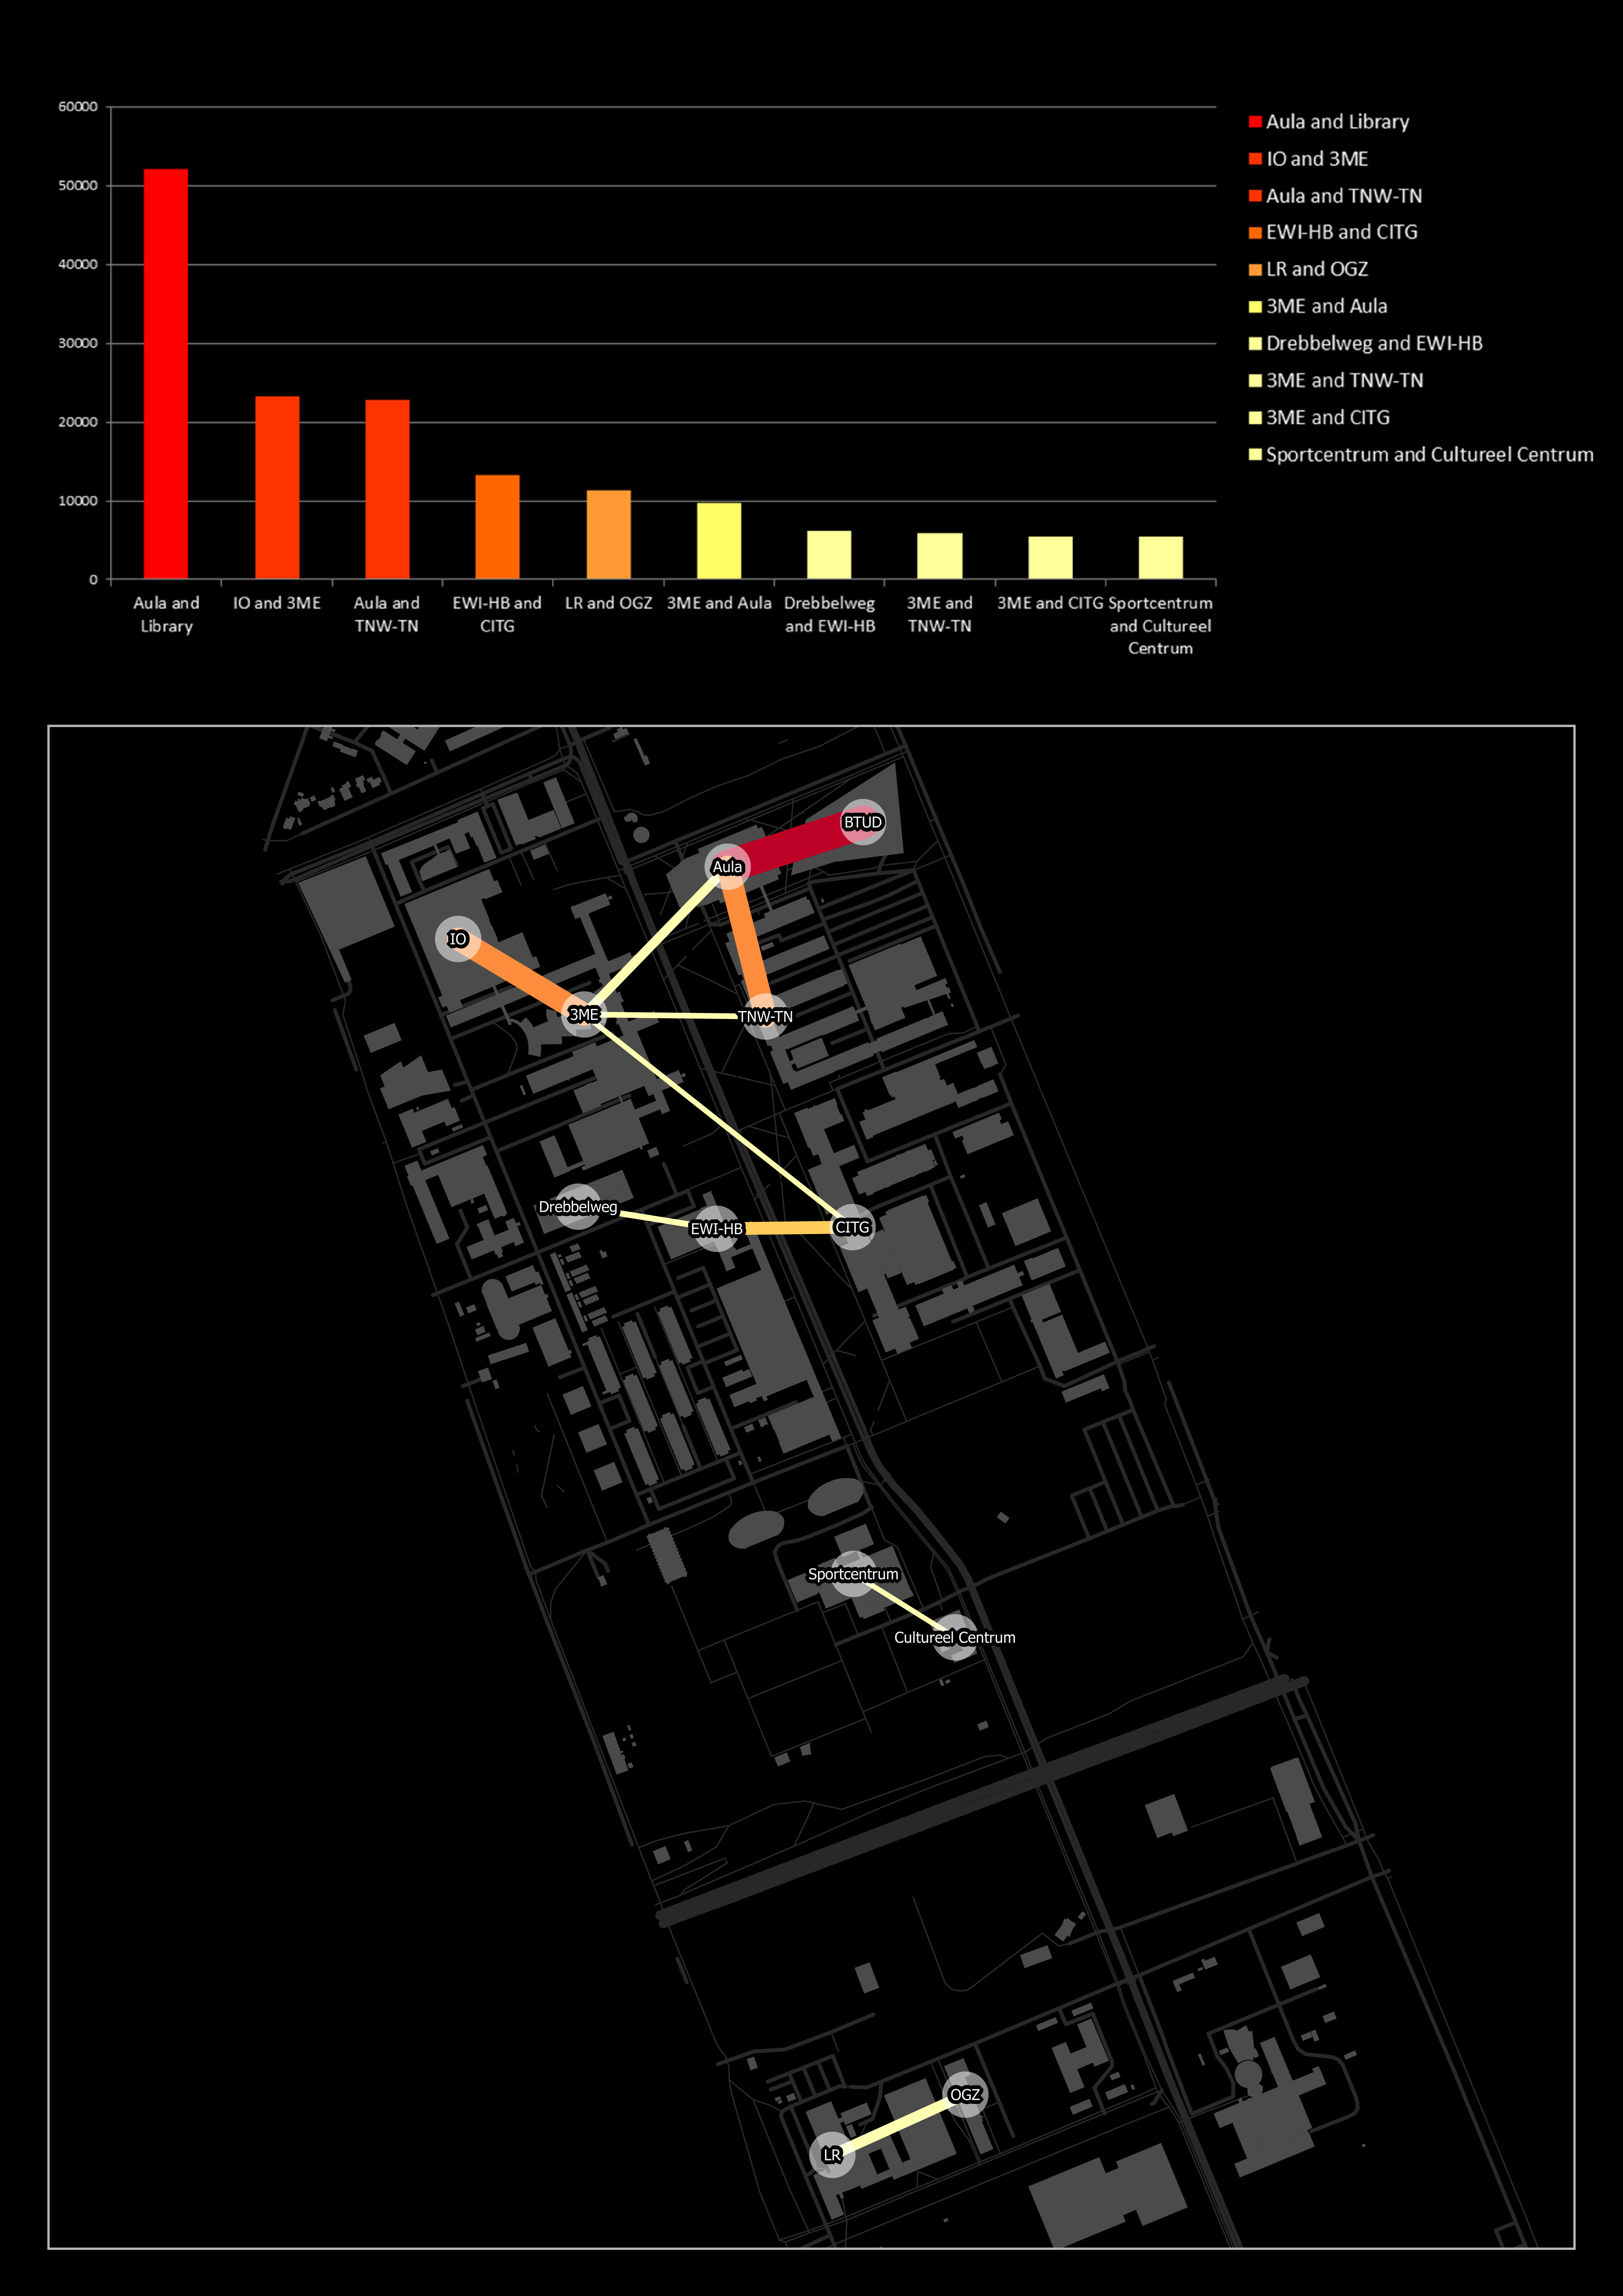
\includegraphics[scale=0.4]{map_total.png}
	\captionsetup{justification=centering}
	\caption{Maps of all movements}
	\label{building_all_map}
\end{figure}
All movements of all time from April 1st to May 27th without filtering static devices is shown above in the graph and map. As it is shown in the graph, there are several peaks at 8:45, 12:45, 13:45, 15:45, 17:45, which are the beginning and the end of the lecture. With 'world', it is clear to see the morning rush hour at around 8:45 when students all come to the campus and around 17:45 when they leave the campus. Not only curve line 'with world', but curve line 'without world' also peaks at these time, which better proves that at these time, many people move on the campus.
The map above shows the top 10 movements on the campus. It is clear that between Aula and library, there are over 50000 movements, which is much more than the others. IO and 3ME, Aula and TNW-TN, EWI-HB and CITG, LR and OGZ, 3ME and Aula, Drebbelweg and EWI-HB, 3ME and TWN-TN, 3ME and CITG, Sportcentrum and Cultureel Centrum are the rest in the top 10. These are building pairs which are more connected and related. People always move between these buildings. So the map actually shows the connectivity of the buildings. It is clear to see that the amount of movements are determined by the locations of the buildings. Normally many movements will happen between two close buildings. Besides, it also depends on the functionality of the buildings. For example, there are many students of EWI having lectures also in CITG, that's why there are many connections between these two buildings.

\subsection{Mobile vs static}\label{chapter9mobilestatic}
\begin{figure}[H]
	\centering
	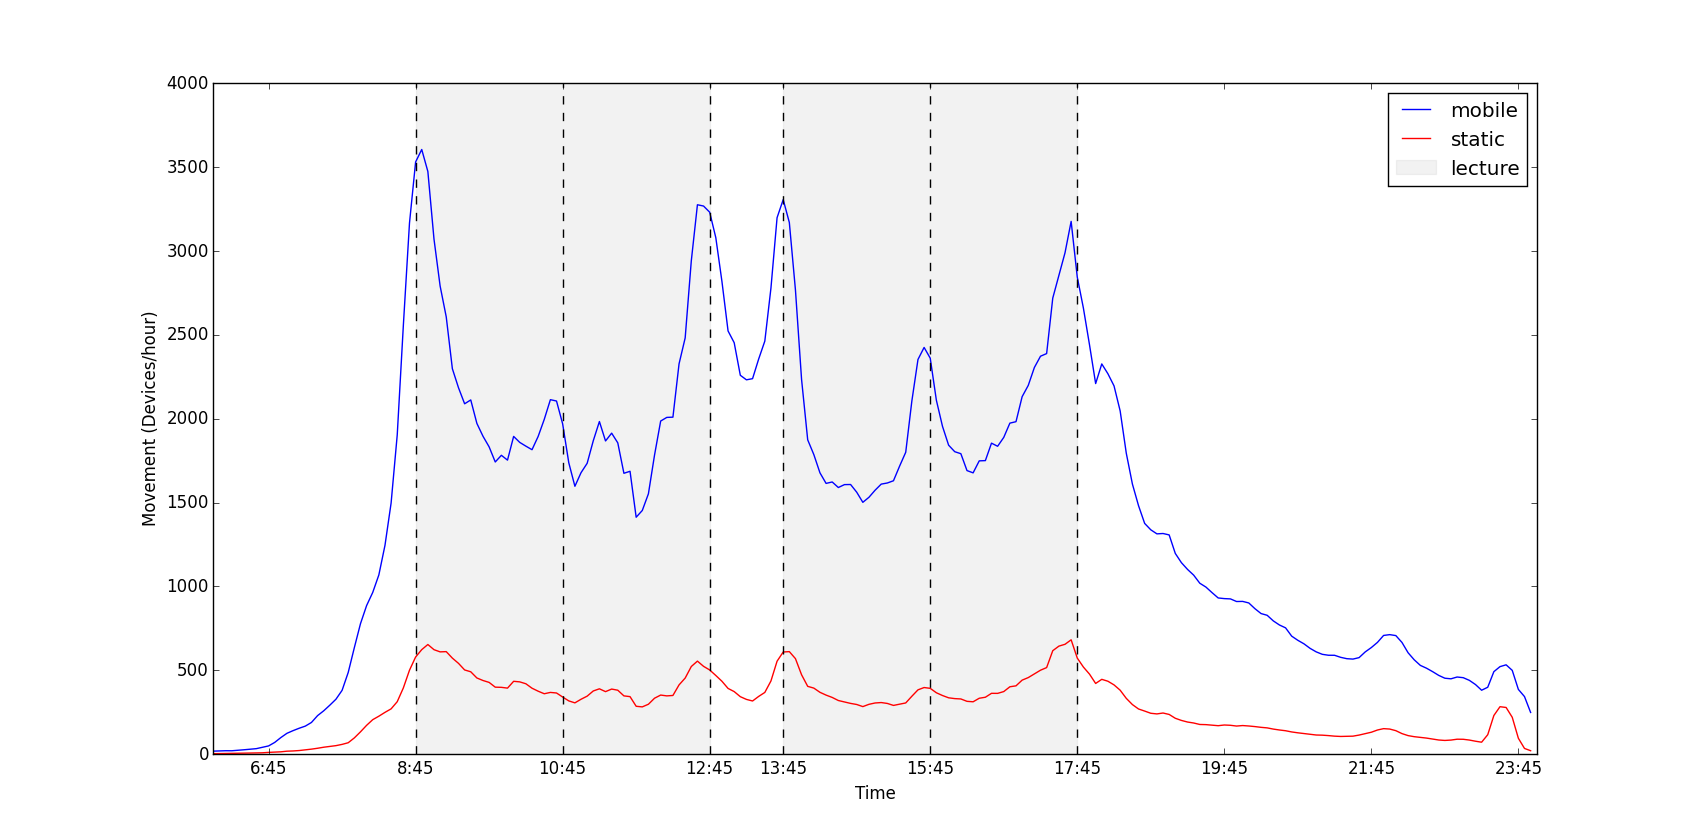
\includegraphics[scale=0.3]{building_mobileStatic_graph.png}
	\captionsetup{justification=centering}
	\caption{Graph of all movements}
	\label{building_mobileStatic_graph}
\end{figure}


\begin{figure}[H]
	\centering
	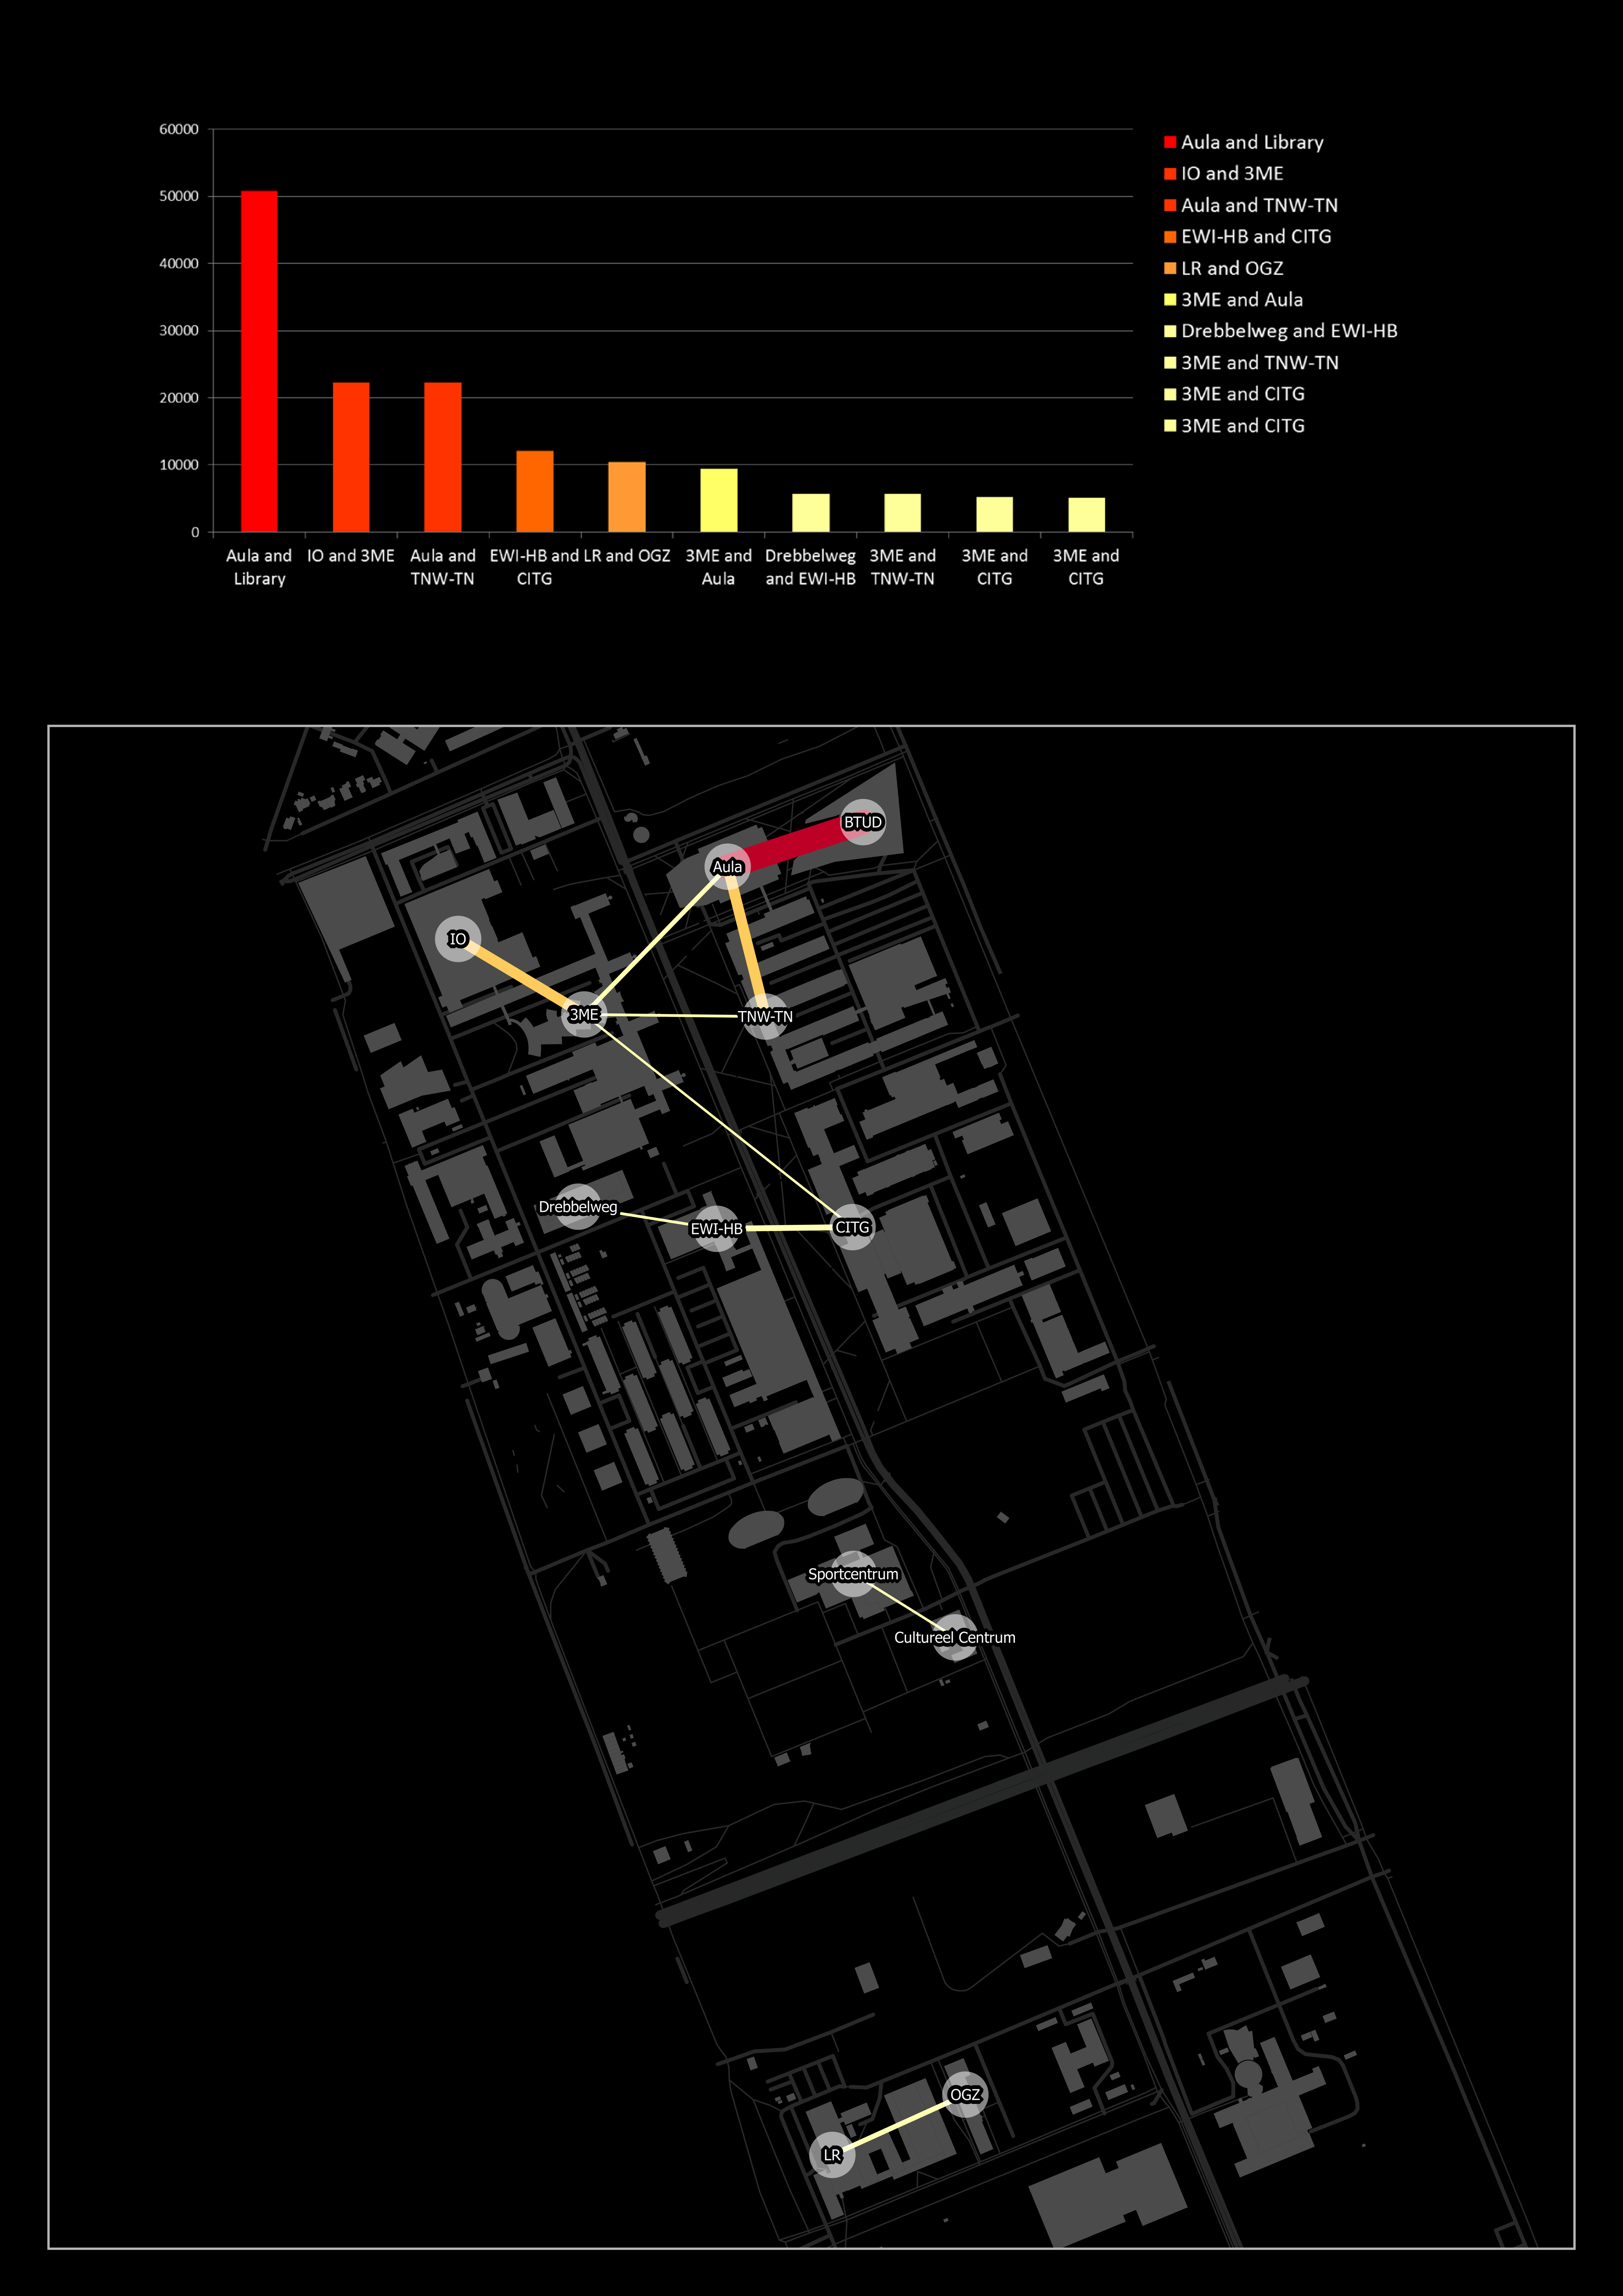
\includegraphics[scale=0.4]{map_mobile.png}
	\captionsetup{justification=centering}
	\caption{Map of mobile device}
	\label{map_mobile_map}
\end{figure}

\begin{figure}[H]
	\centering
	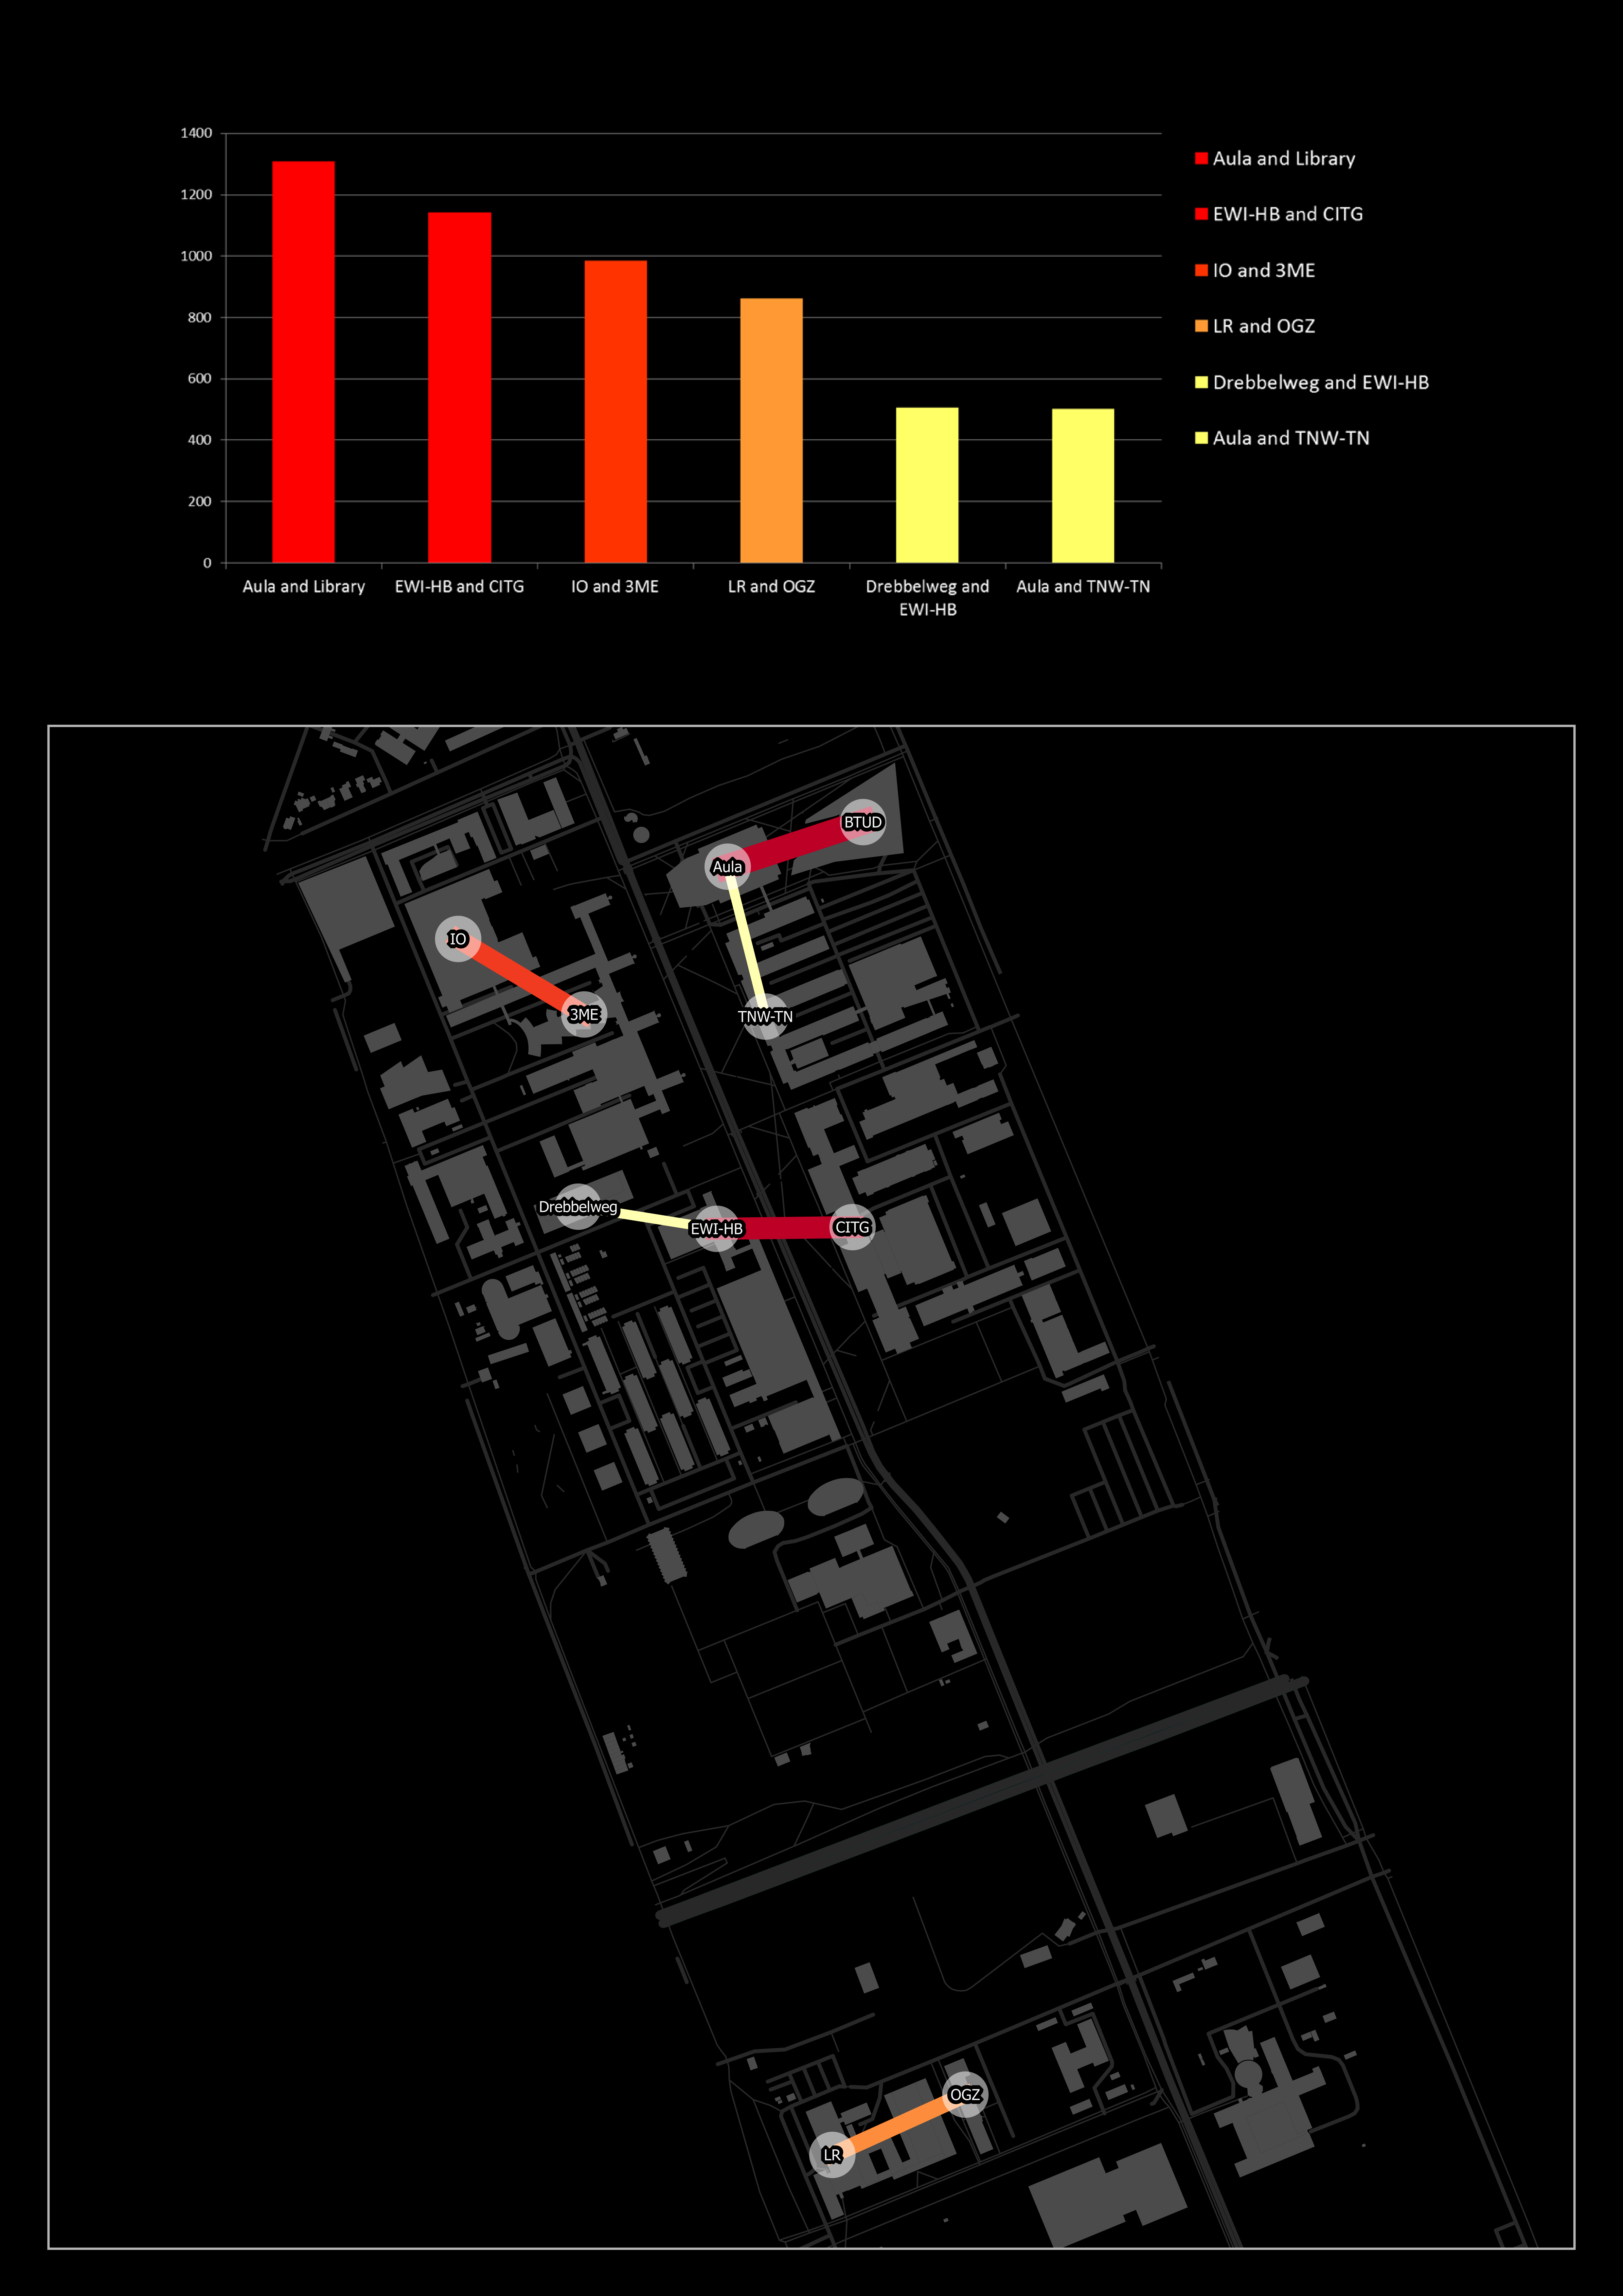
\includegraphics[scale=0.4]{map_static.png}
	\captionsetup{justification=centering}
	\caption{Map of static}
	\label{map_static_map}
\end{figure}
The graph (\autoref{building_mobileStatic_graph}) shows the difference between mobile and static devices. It is obvious that compared with peaks of mobile devices, the peaks of static device are more flat, which indicates that mobile devices are more mobile than static devices. It also implicitly proves the correctness of the classification of mobile device and static device.
In the two maps, \autoref{map_mobile_map} and \autoref{map_static_map}, mobile devices move between library and aula much more than the other buildings and in the map of static device, the difference is not as much.
\subsection{Week vs weekend}\label{chapter9weekweekend}
\begin{figure}[H]
	\centering
	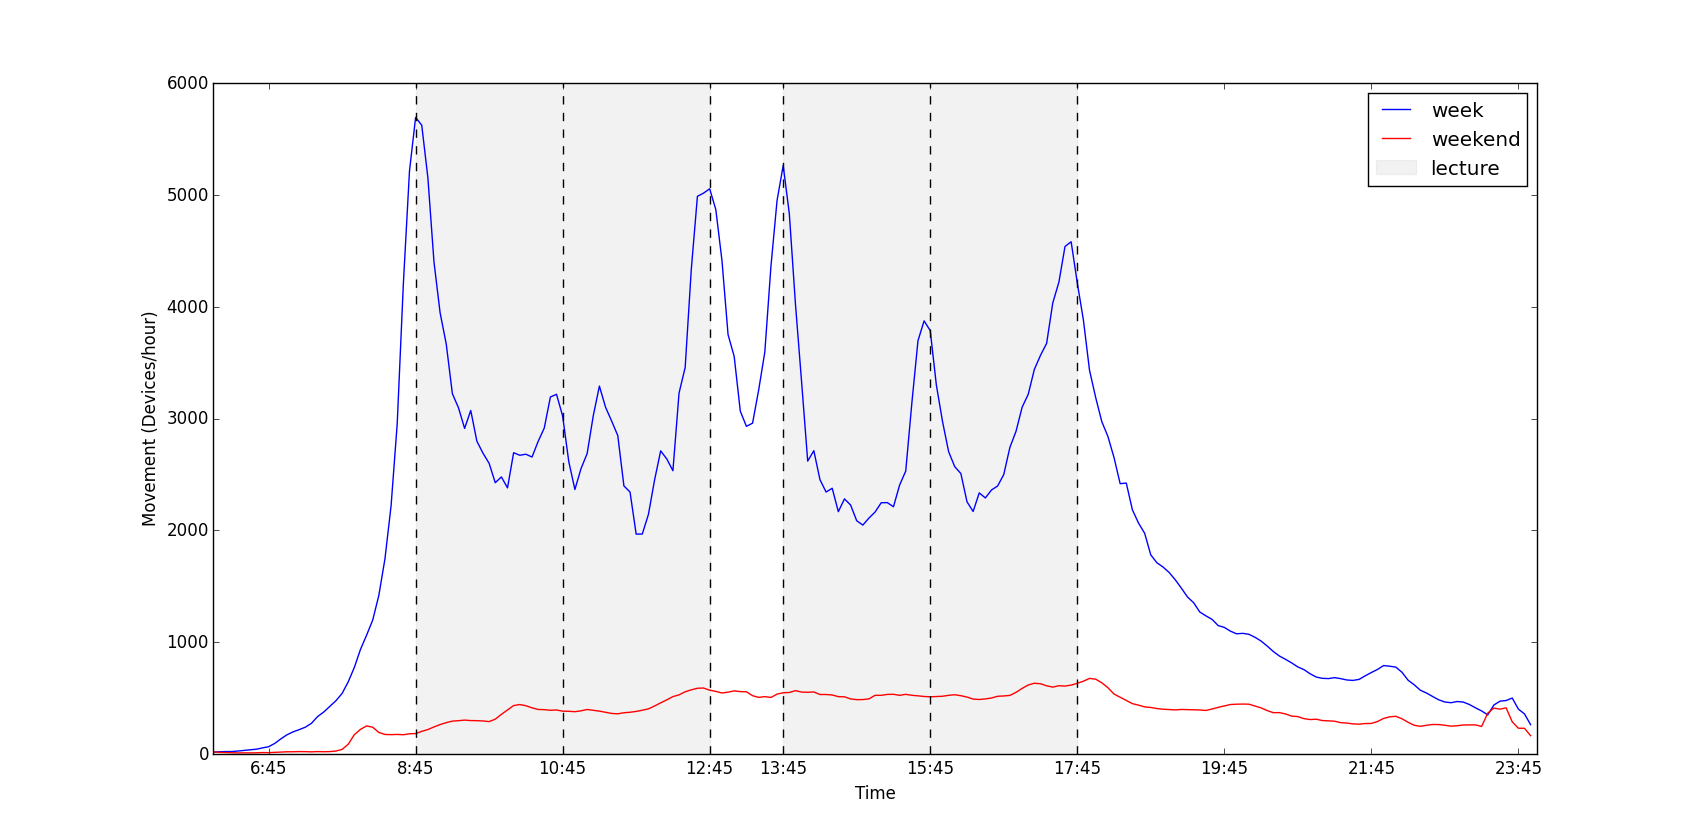
\includegraphics[scale=0.3]{building_weekWeekend_graph.png}
	\captionsetup{justification=centering}
	\caption{Graph of weekdays and weekends}
	\label{building_weekWeekend_graph}
\end{figure}


\begin{figure}[H]
	\centering
	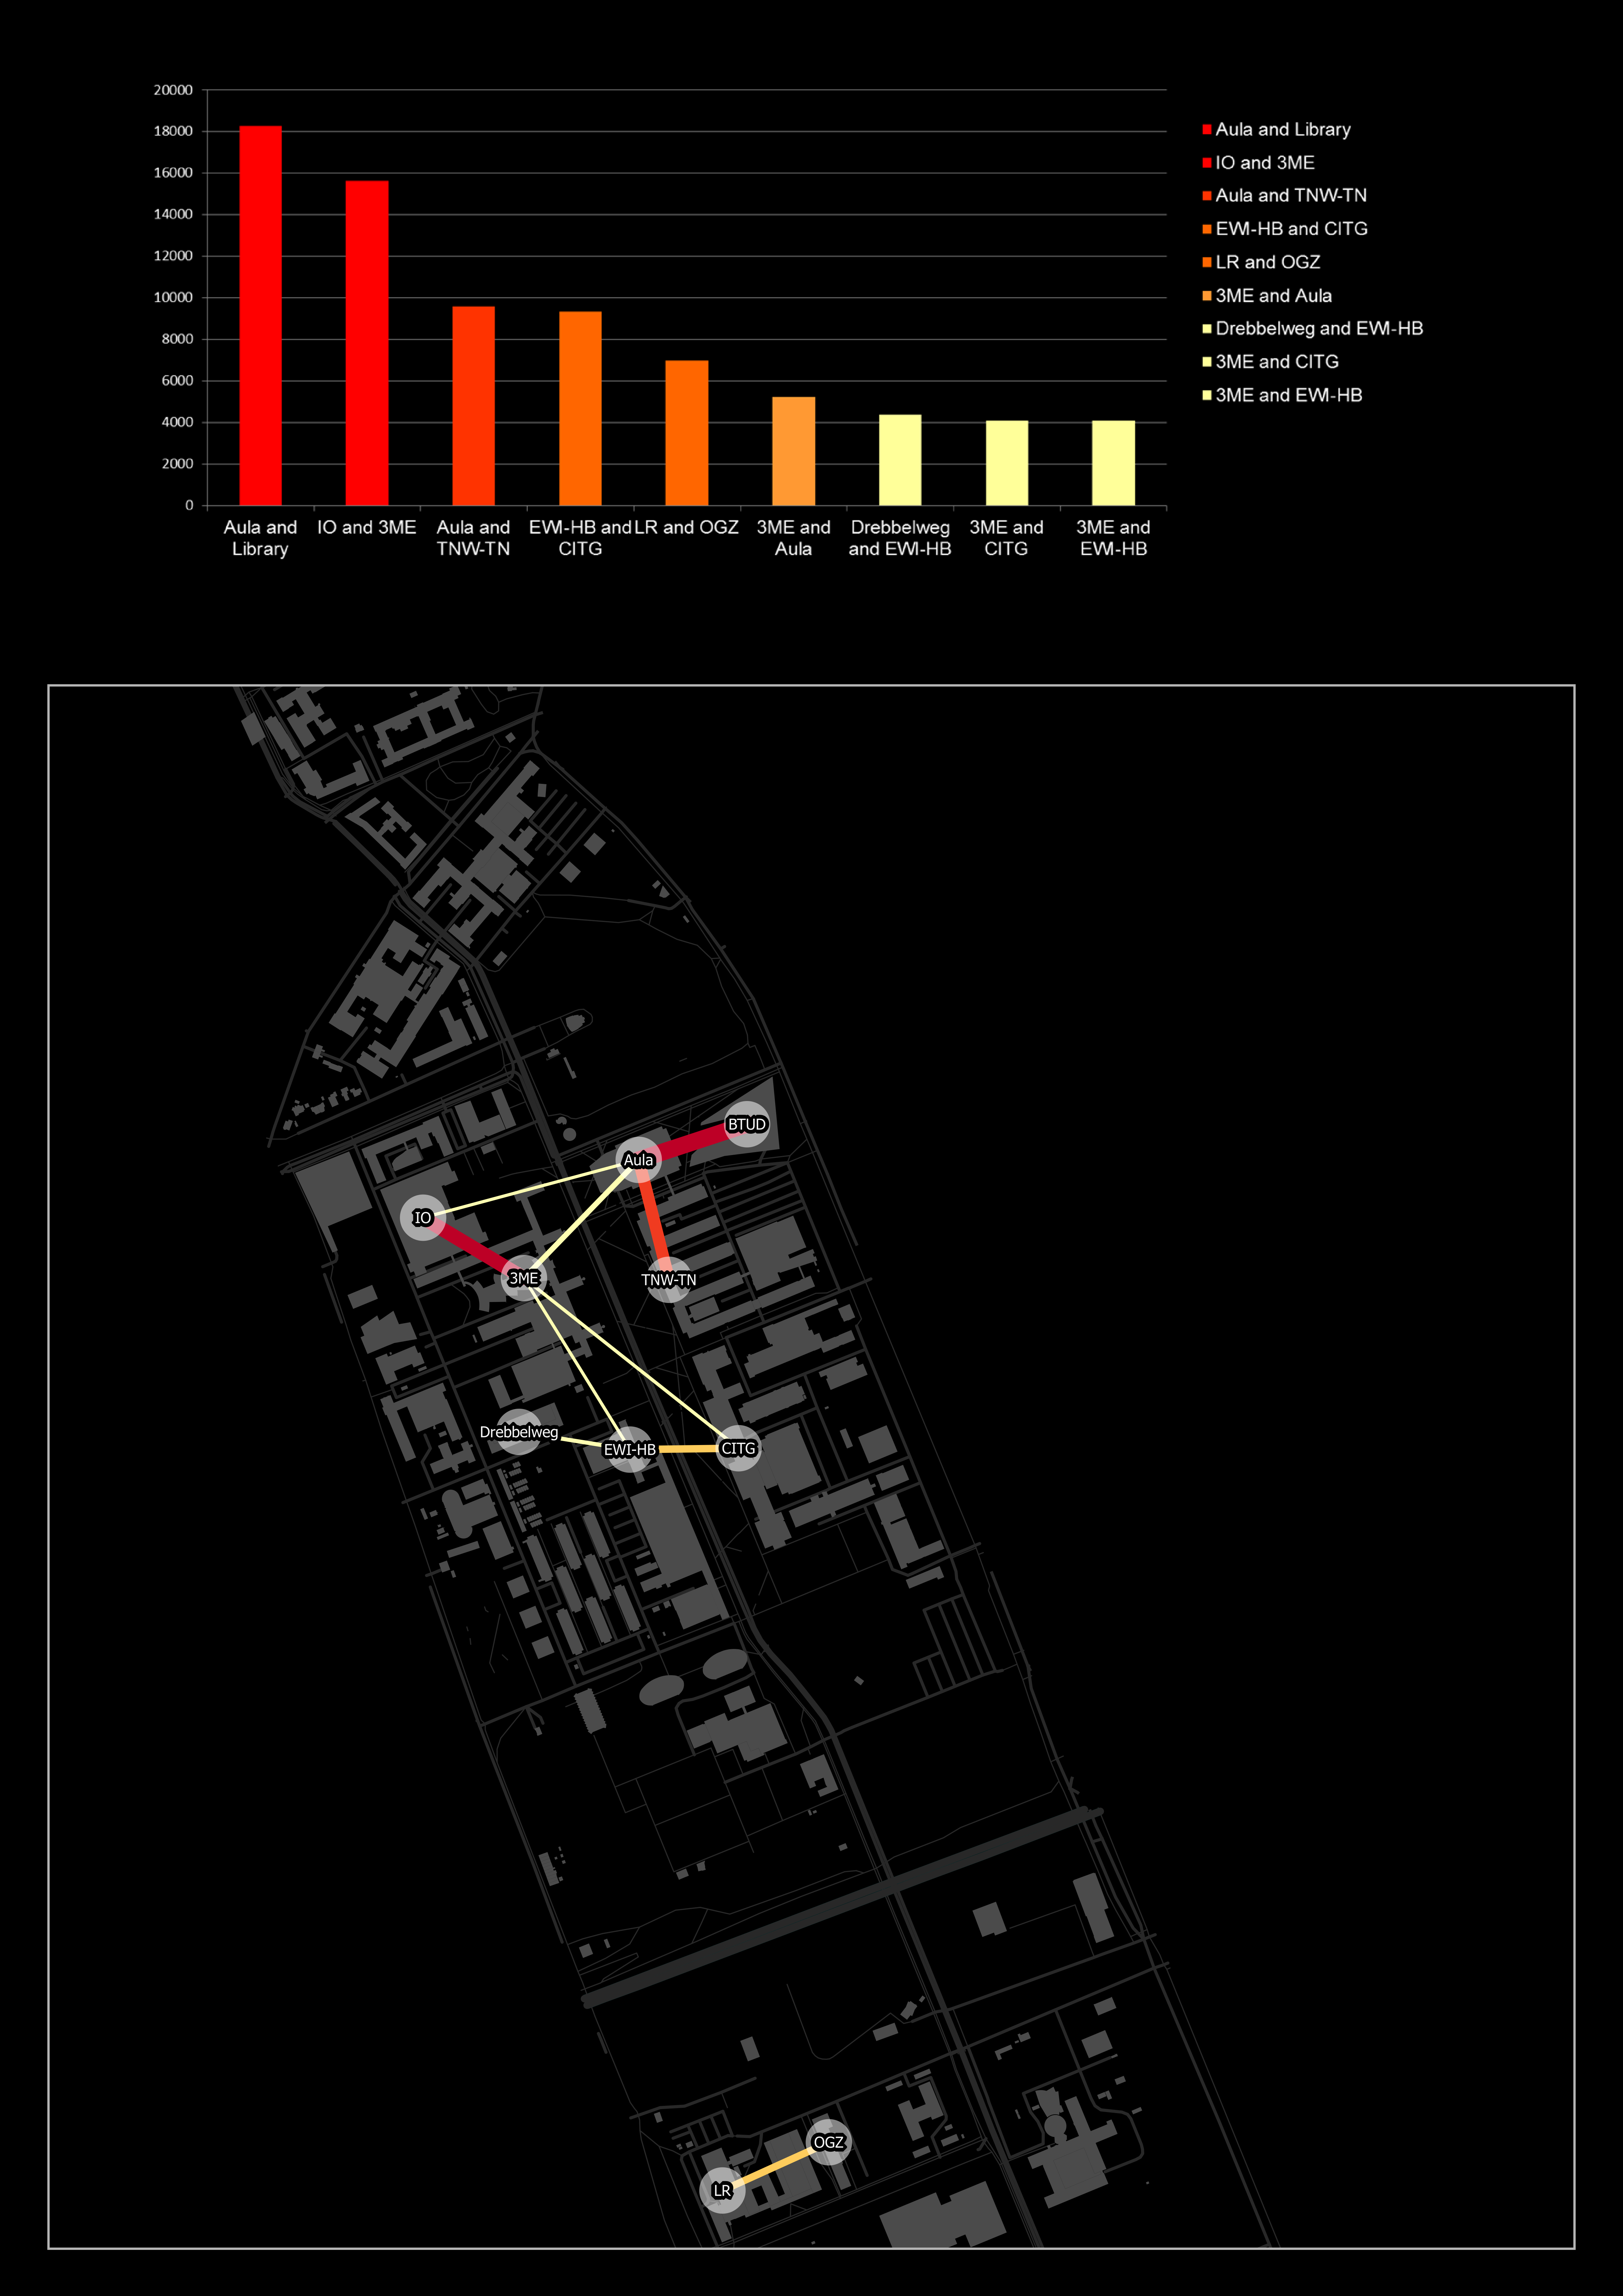
\includegraphics[scale=0.4]{map_weekdays.png}
	\captionsetup{justification=centering}
	\caption{Map of weekdays}
	\label{weekdays_map}
\end{figure}

\begin{figure}[H]
	\centering
	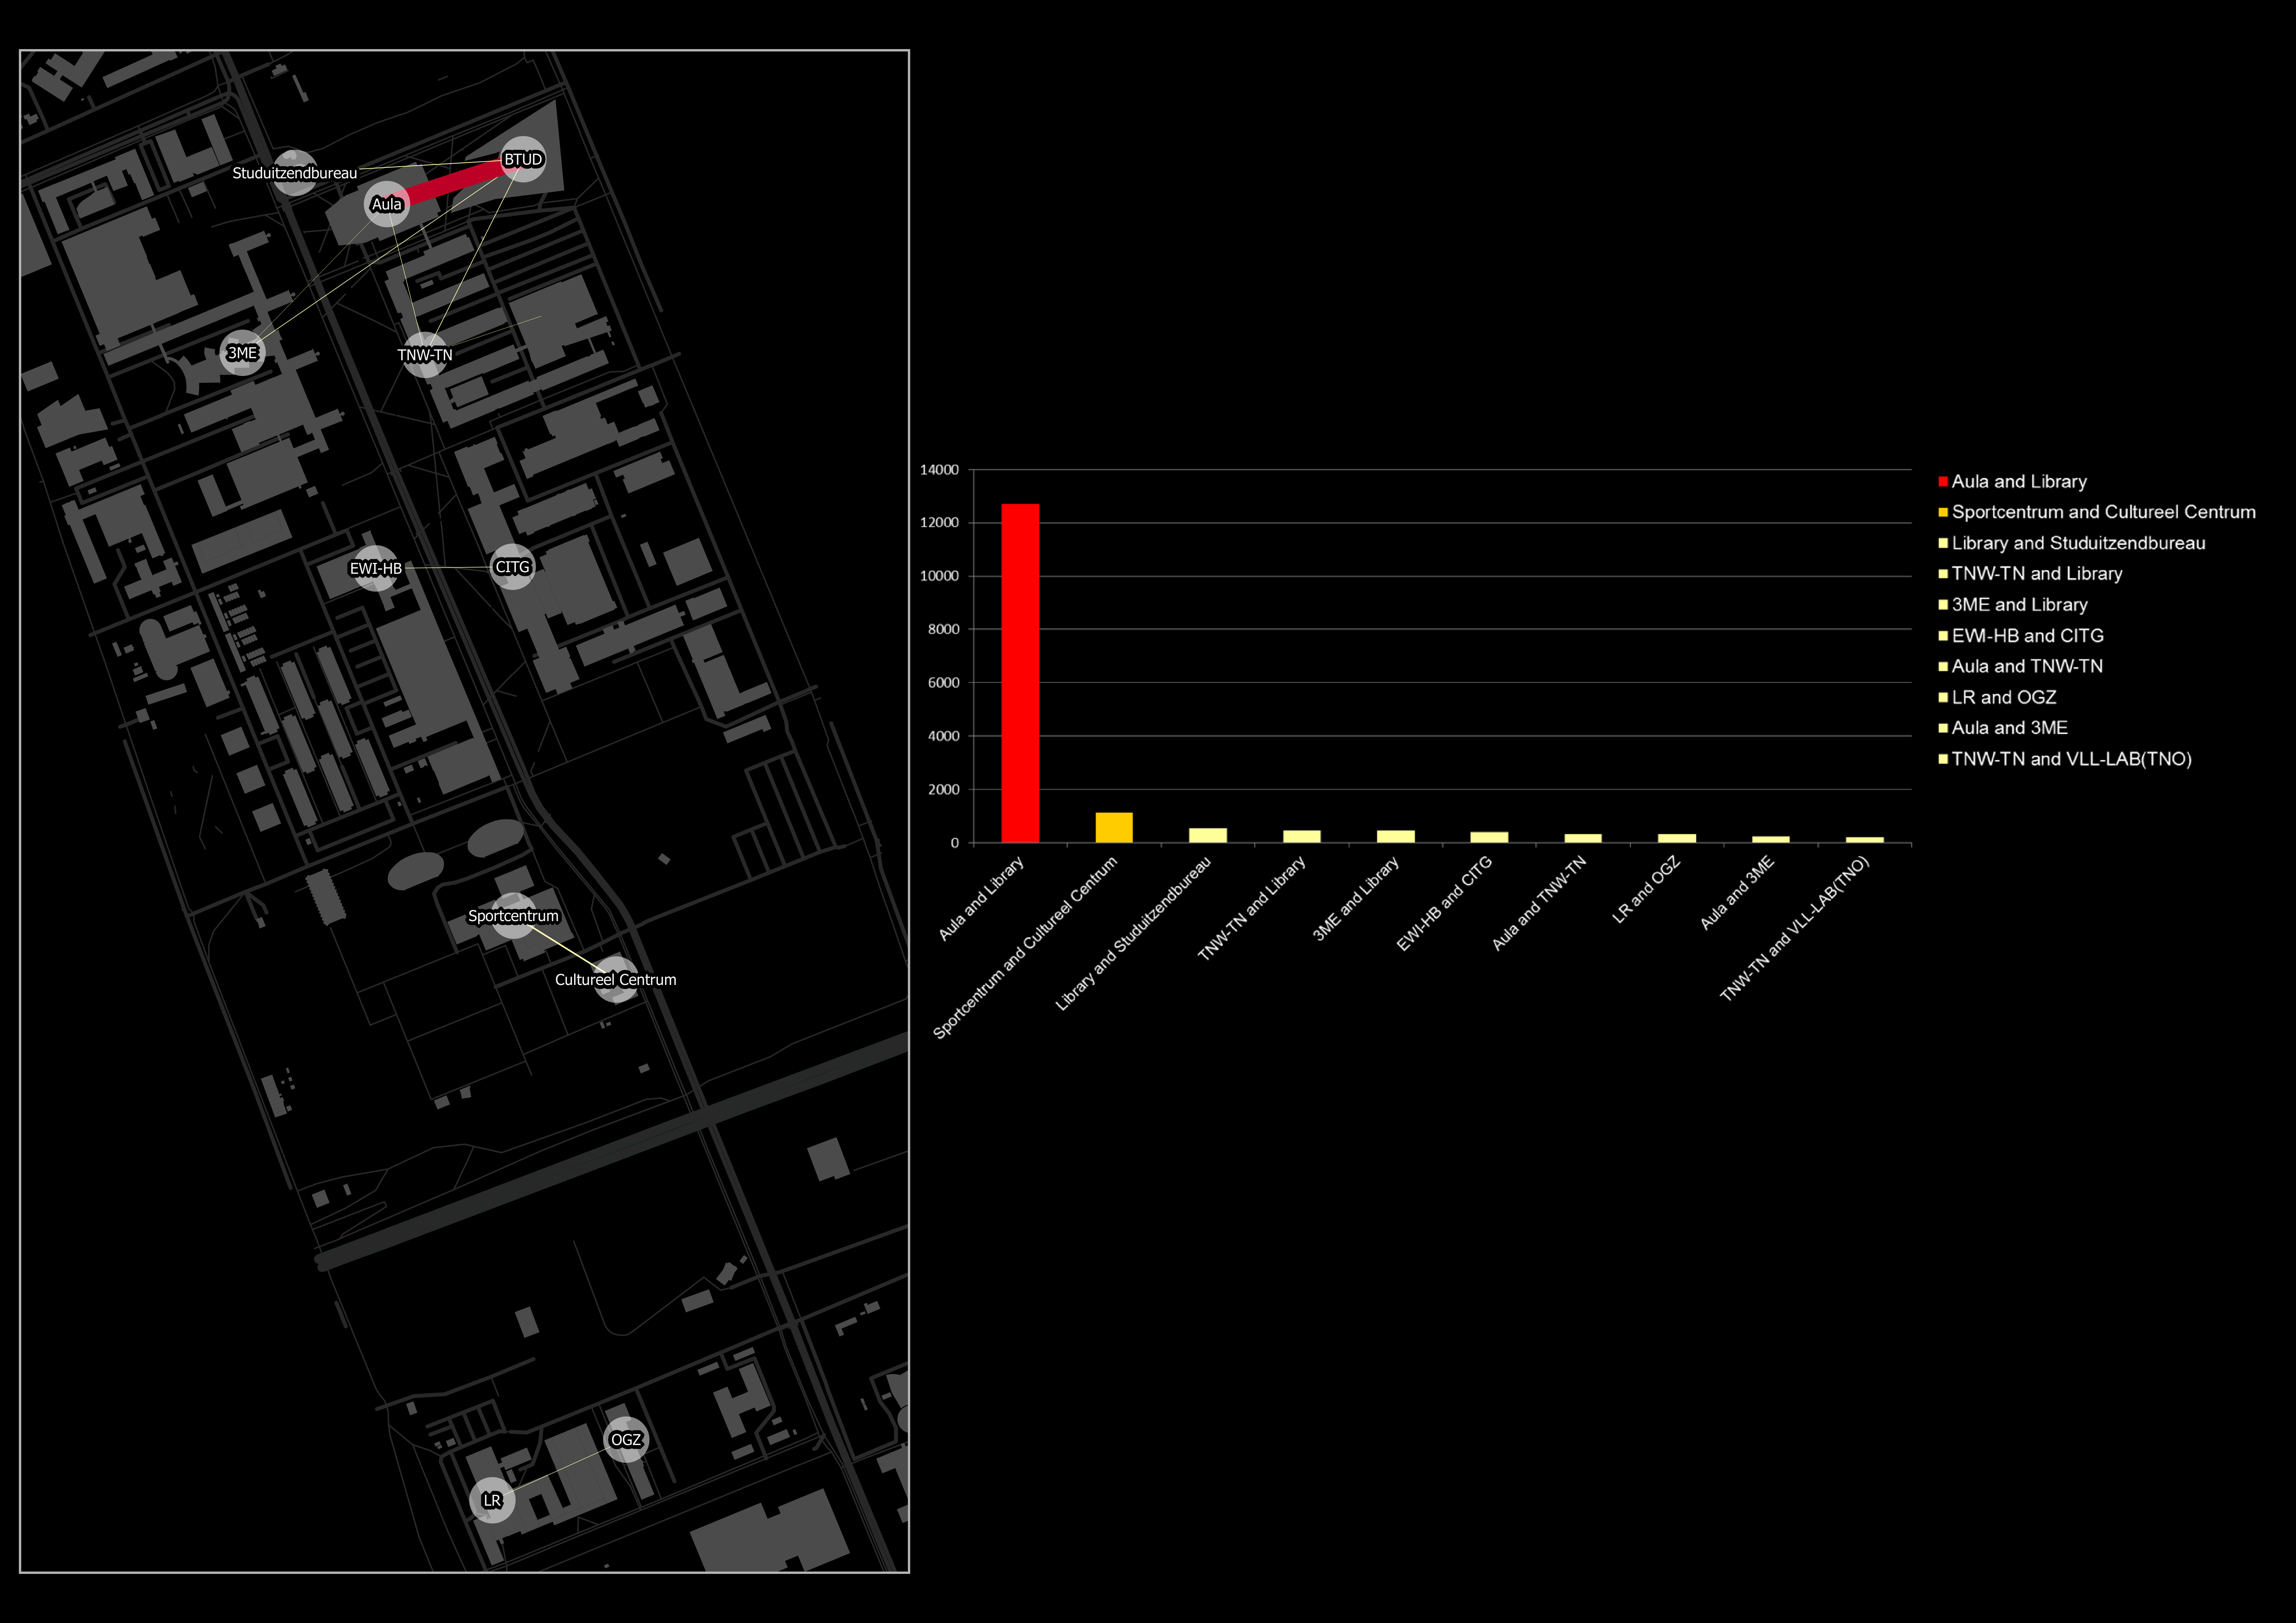
\includegraphics[scale=0.4]{map_weekends.png}
	\captionsetup{justification=centering}
	\caption{Map of weekends}
	\label{weekends_map}
\end{figure}
The \autoref{building_weekWeekend_graph} shows the different movement patterns in weekdays and on weekends. It is clear that in weekdays, the movements are more regular, the peaks of movements match the lecture time very well, however on weekends, the movements are much less and also less regular than weekdays. On weekends. the curve line is flat, indicating that people move on the campus more casually.
The map of weekdays(\autoref{weekdays_map}) is similar to all movements map(\autoref{building_all_map}), but the movement between sportcentrum and culureel centrum is no longer in the top 10 movements. However in the map of weekends(\autoref{weekends_map}), there are far more movements between aula and library, and sportcentrum and culureel centrum is top 2. Compare these two maps, it is also clear that more people go to sportcentrum and culureel centrum on weekends.

\subsection{From and to}\label{chapter9fromto}
\begin{figure}[H]
	\centering
	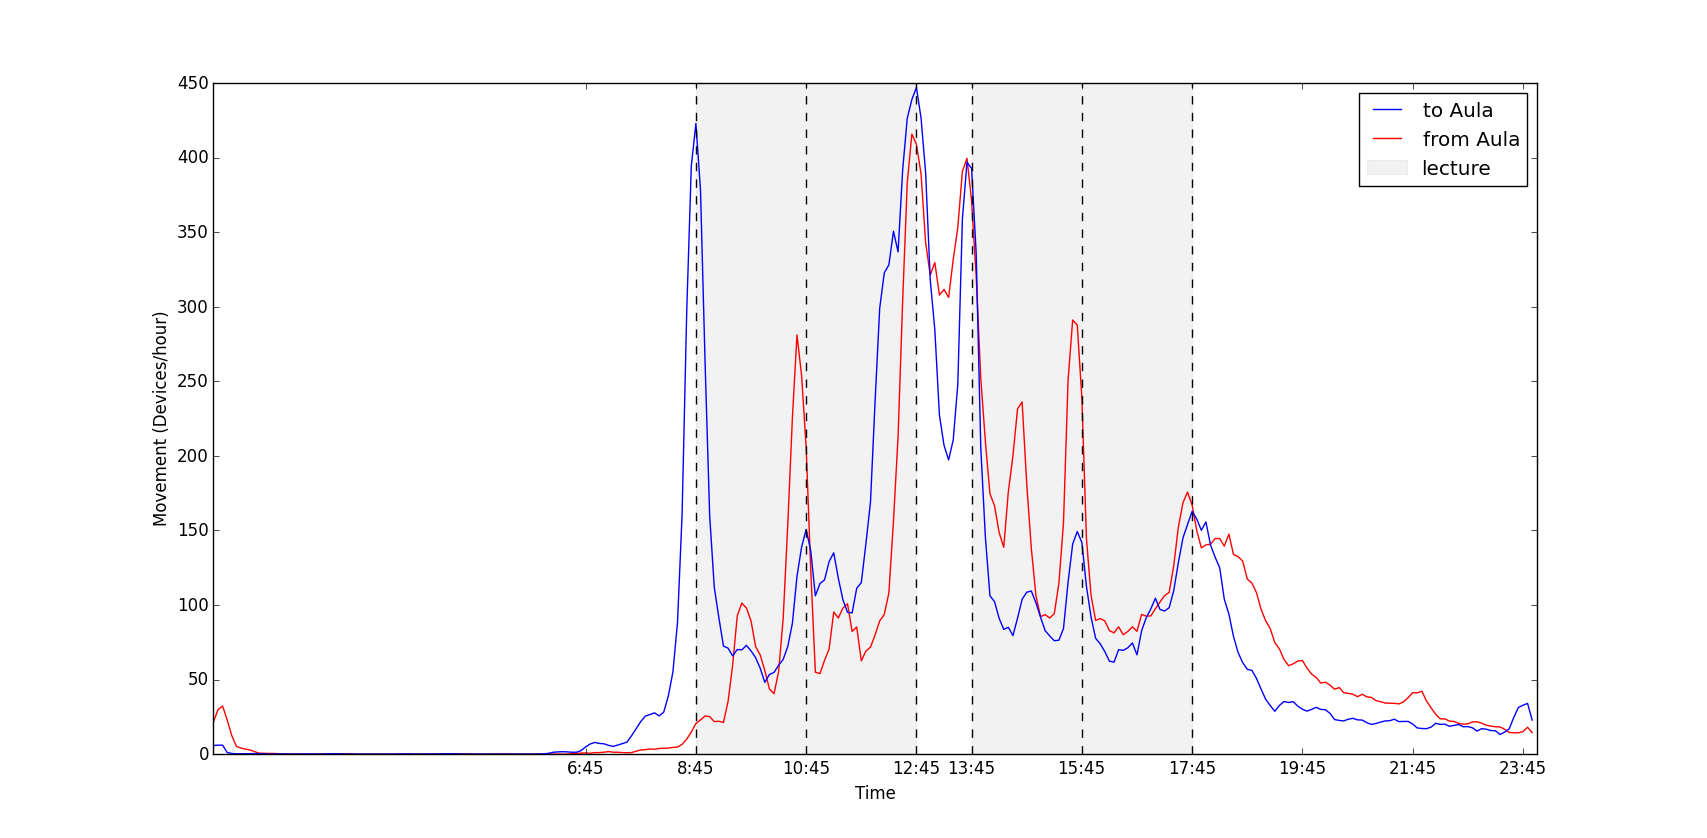
\includegraphics[scale=0.3]{building_fromTo_aulaGraph.png}
	\captionsetup{justification=centering}
	\caption{Graph of weekdays and weekends}
	\label{building_weekWeekend_graph}
\end{figure}


\begin{figure}[H]
	\centering
	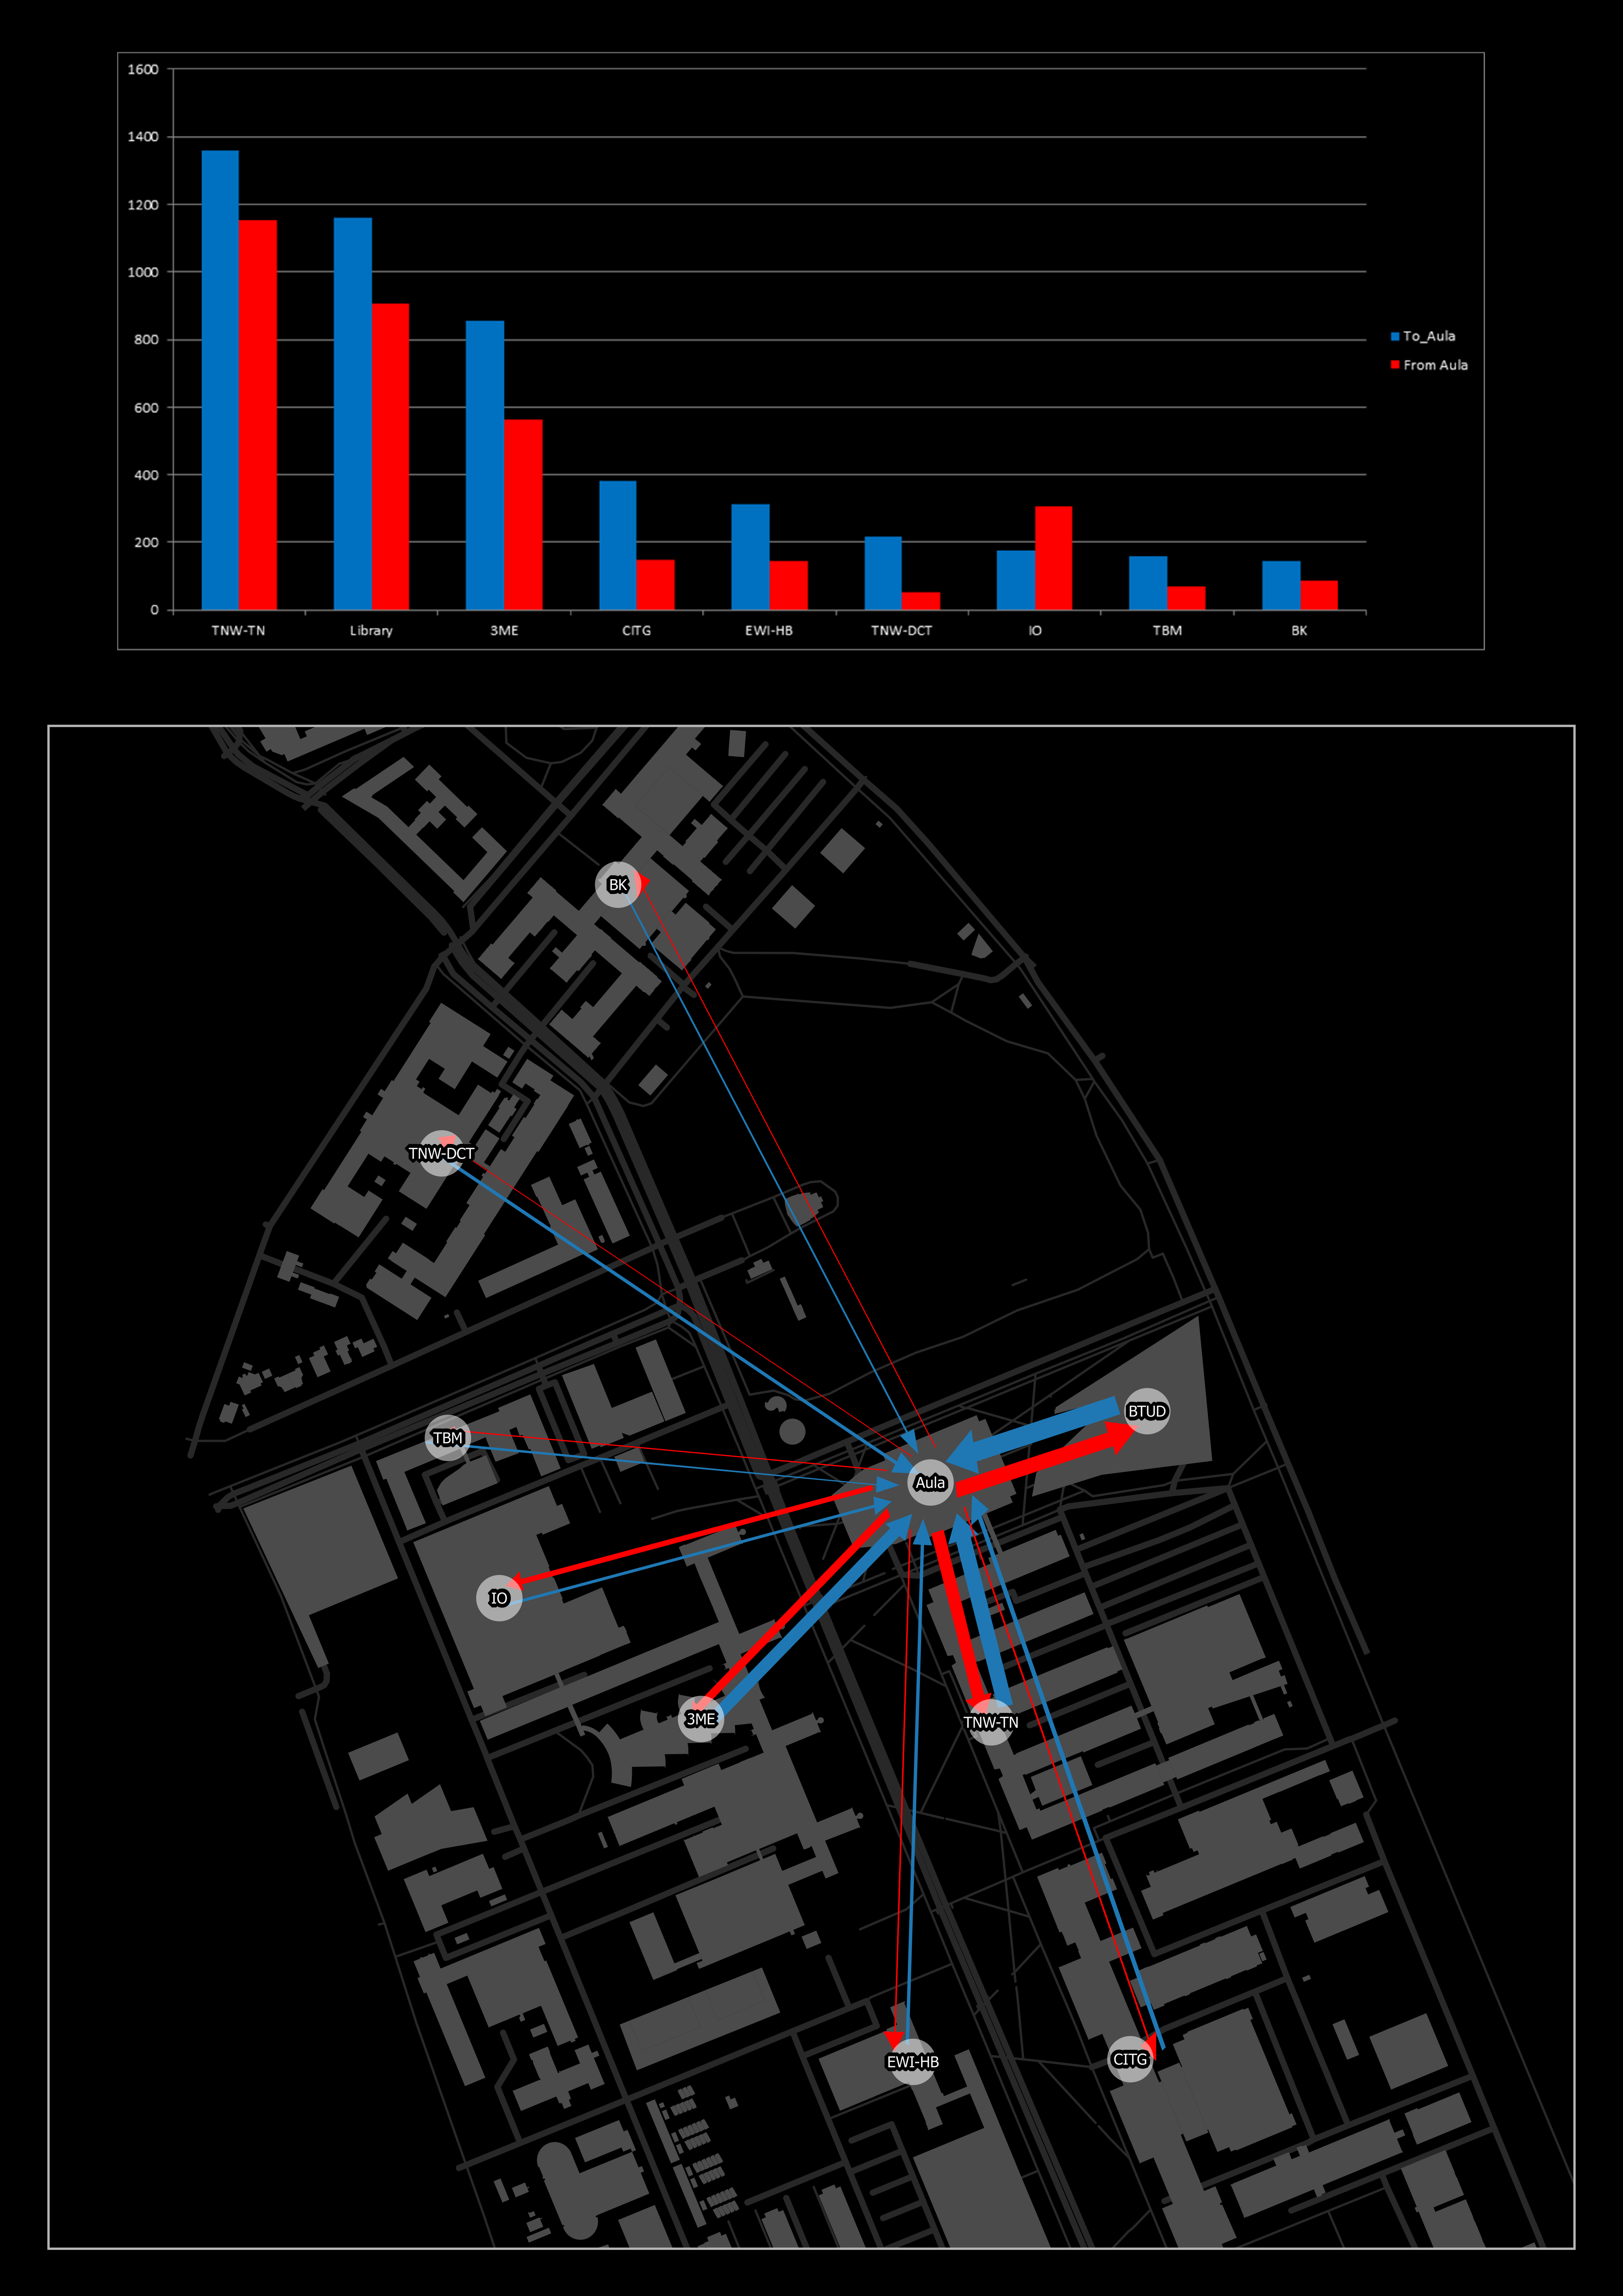
\includegraphics[scale=0.4]{map_1215to1300_Aula.png}
	\captionsetup{justification=centering}
	\caption{Map of from or to Aula between 13:15 to 14:00}
	\label{12151300_map}
\end{figure}

\begin{figure}[H]
	\centering
	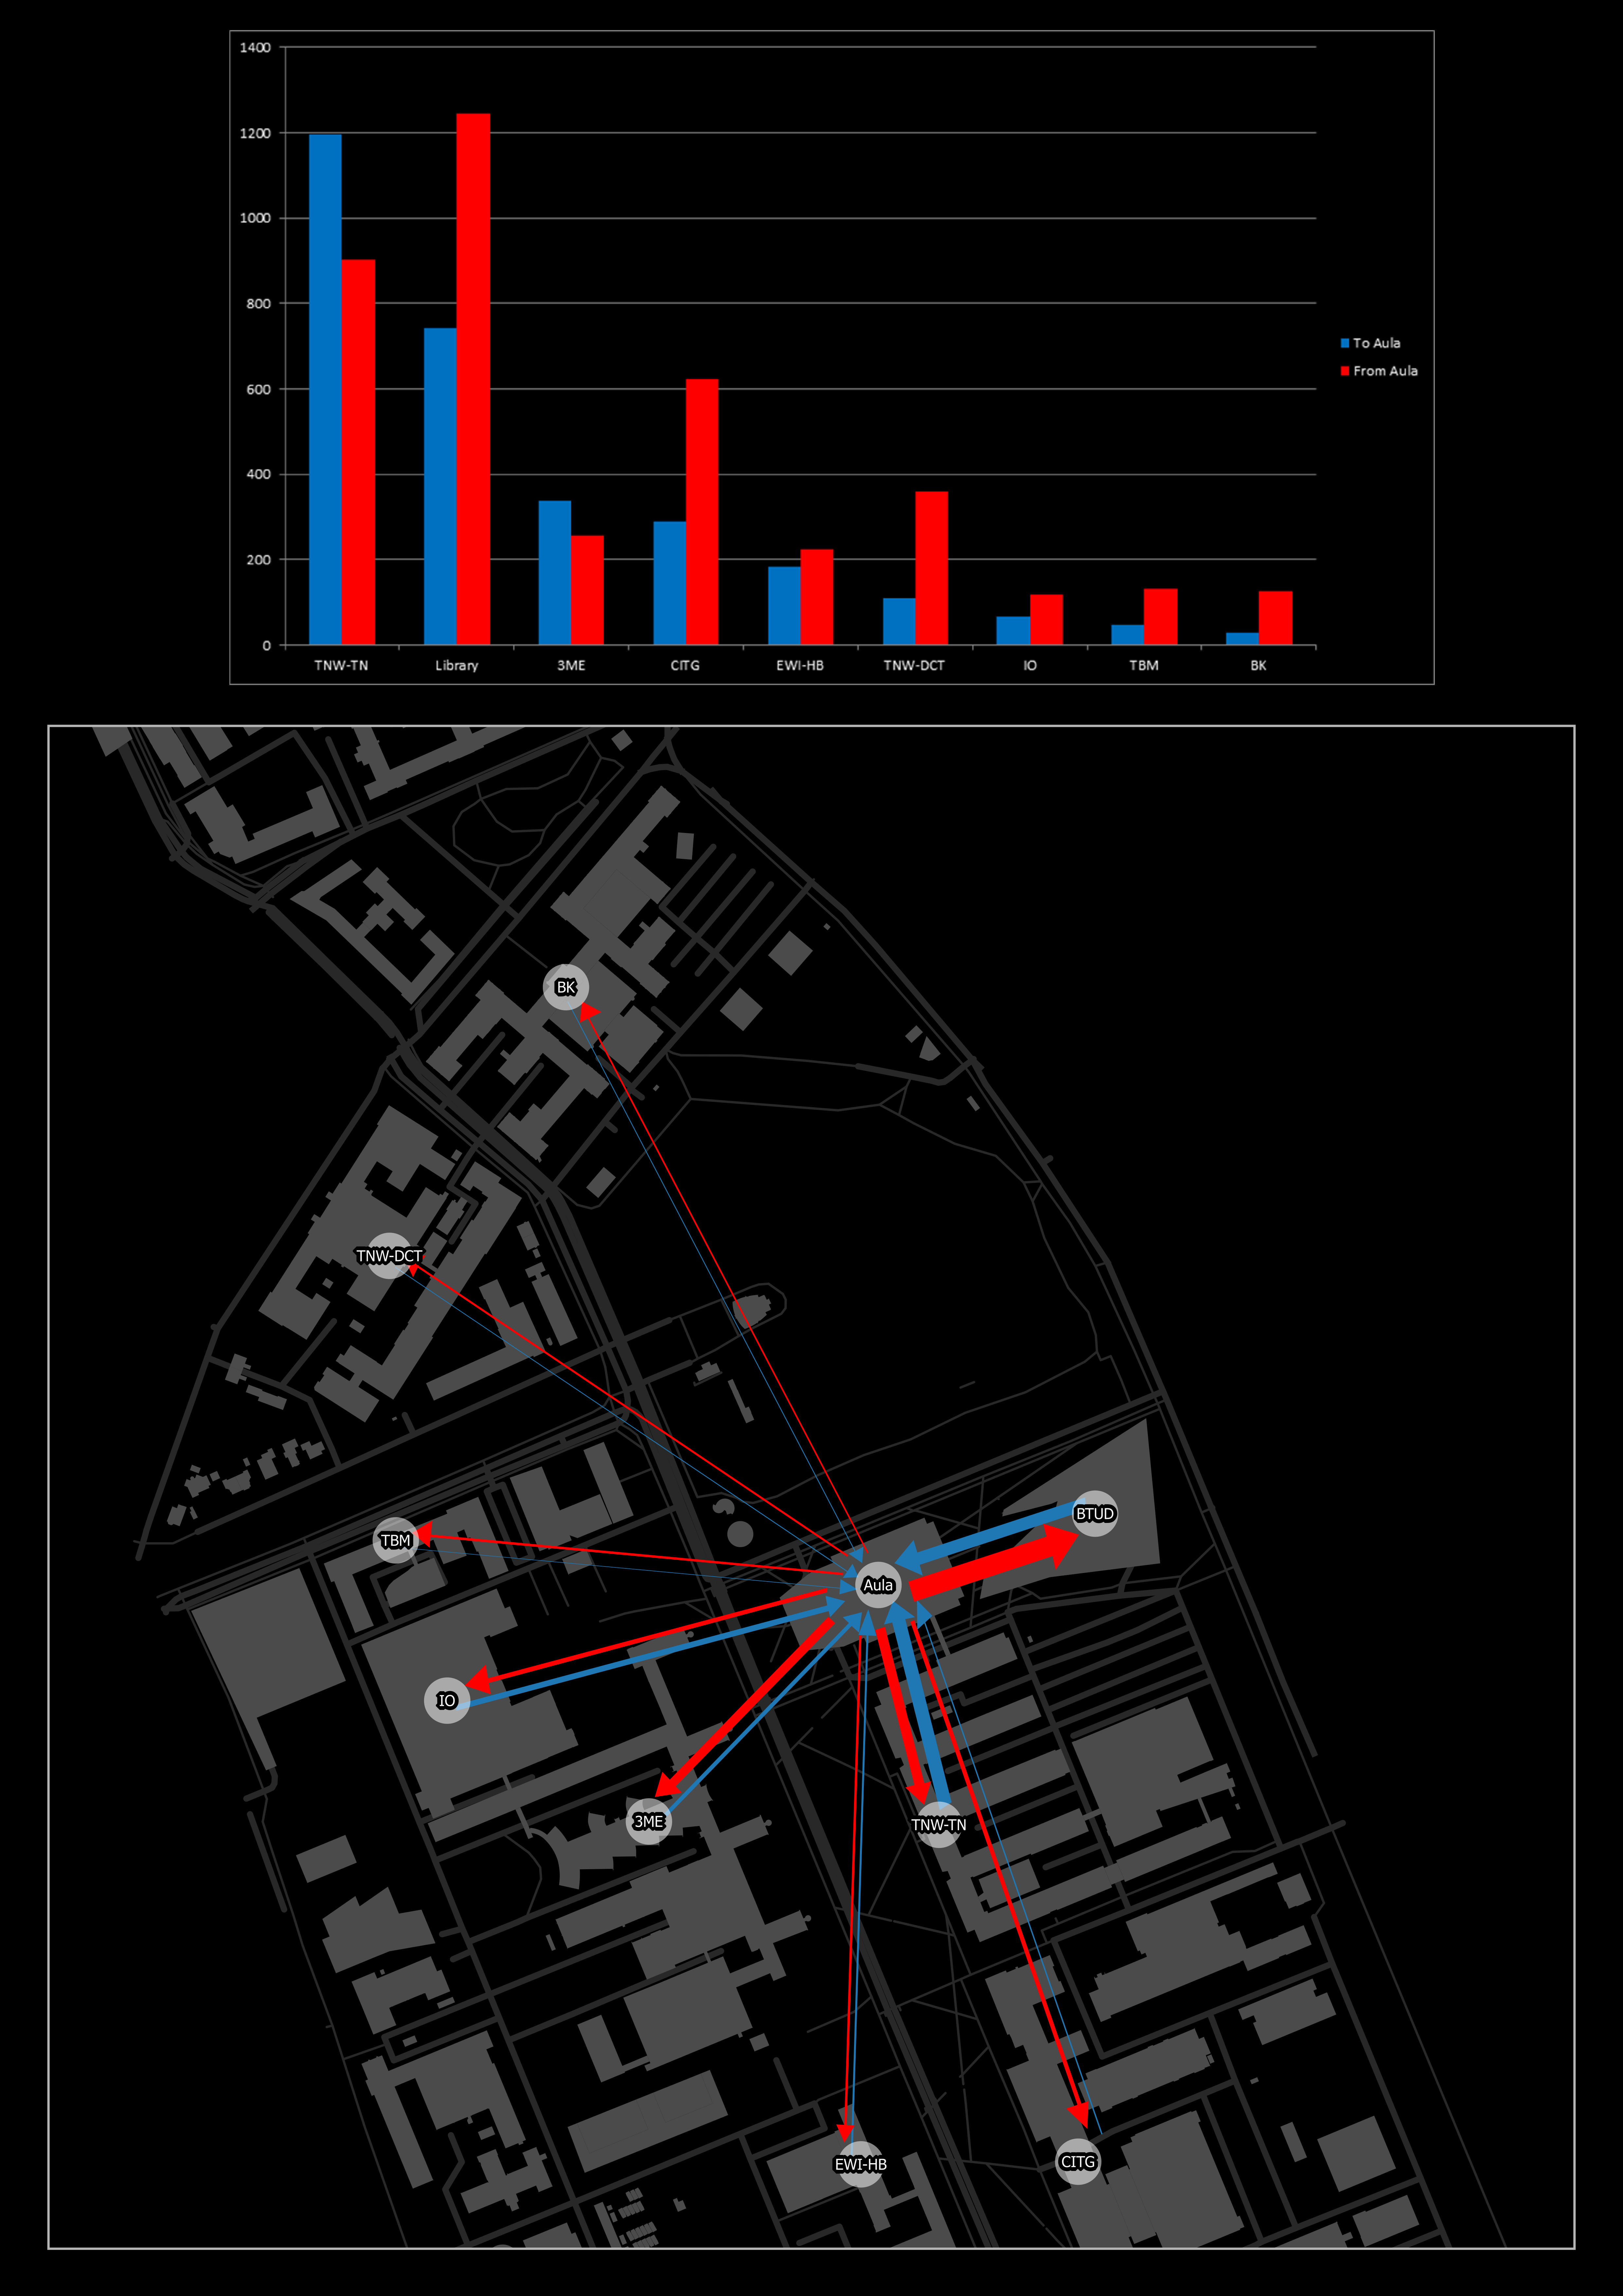
\includegraphics[scale=0.4]{map_1315to1400.png}
	\captionsetup{justification=centering}
	\caption{Map of from or to Aula between 13:15 to 14:00}
	\label{13151400_map}
\end{figure}
The graph shows the movements from and to Aula in time. At 8:45, there are many movements to Aula, the reason might be that there are also lectures in Aula at this time. And many people leave at 10:45 when the lectures end. During lunch time between 12:15 to 14:00, there are almost the same amount of people moving to and from Aula.
The above two maps respectively show the movements from and to Aula from 12:15 to 13:00 and from 13:15 to 14:00. They show that people from which faculties go to Aula for lunch most.
Most people go from TNW-TN to Aula, from library to Aula and from 3ME to Aula. Also some people go from CITG, EWI-HB, TNW-DCT, IO, TBM, BK for lunch. In general, more people move to Aula than from Aula between 12:15 and 13:00. From 13:15 to 14:00, more people move from Aula to other buildings especially library. The buildings in \autoref{12151300_map} match the buildings in \autoref{13151400_map}, which to some degree proves that people from these faculties do use Aula as canteen during lunch time.